\chapter{相关研究现状分析}


\section{数据立方的计算研究}

数据立方的计算涉及到对原事实表数据进行扫描,对相应的 GroupBy 属性值执行聚合计算以及生成相应的立方数据等几个步骤。在立方计算的问题讨论中,如何尽可能地减少原事实表的数据扫描次数、降低 I/O 代价以及内存的开销,成为评价一个立方计算方法高效性的几个关键要点。

GBLP \cite{gray1997data}、PipeSort、PipeHash \cite{agarwal1996computation}、BUC \cite{beyer1999bottom} 以及 Partitioned-Cube \cite{ross1997fast} 是几种经典的数据立方计算方法。 其中GBLP、 PipeSort、 PipeHash以及Partitioned-Cube 均是自顶向下的计算,而 BUC 则是自底向上的计算方法。如图 \ref{4_dimension_lattice},展示了一个 4 维数据立方的 lattice,其中 A,B,C,D 均为属性维度。在一个数据立方的 lattice 中,每一个节点代表一个region,箭头从父节点指向子节点。自顶向下,顾名思义就是在一个 lattice 中从父节点开始往下计算,而自底向上则相反。

\begin{figure}[!htb]
\centering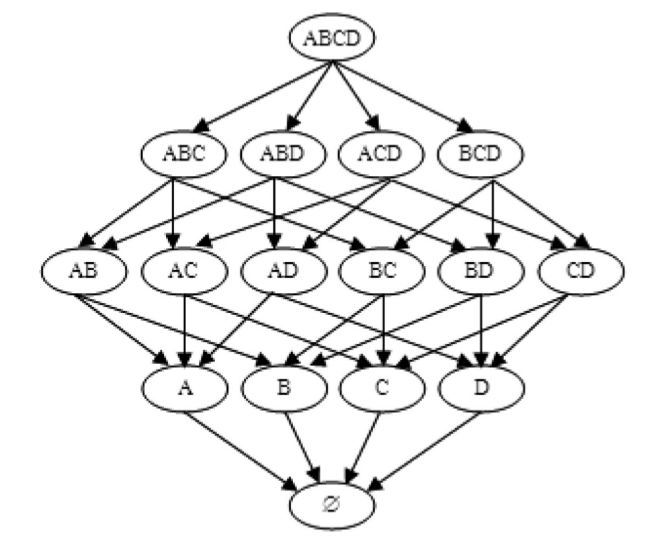
\includegraphics[width=3in]{picture/ch_current_research/4_dimension_lattice} 
\caption{4维数据立方的Lattice}\label{4_dimension_lattice} 
\end{figure} 

\subsection{GBLP}

Jim Gary 等人在提出数据立方概念的同时,还提出了一种计算数据立方的算法 —— GBLP[12]。该算法的核心思想是自顶向下,为每个region选择其最小的父region(指region内group数量最少的region)作为其计算的基础。对于一个 lattice,越往下,region内group的数量就会变得越少,因此相对于每个region都基于原始数据表进行计算,基于最小父region的计算能因为数据量的大规模减少而加快了一个region的计算速度。但该方法只是把一个 lattice 修剪成一个树型结构,却没有提供一个特定的 lattice 遍历计划。另外当计算数据量很大无法完全存储于内存时,该方法没有提供一个有效的磁盘访问策略,这使得该方法的 I/O 代价会很高。

\subsection{PipeSort}

1996 年,Agarwal 等人针对 GBLP 算法的缺陷,提出了第一个改进的数据立方计算方法 —— PipeSort\cite{agarwal1996computation} 。在一个 lattice 中,假如一个子region的维属性排序顺序是它其中一个父region的维属性排序顺序的前缀,则该子region可以在其父region的基础上计算而无需额外的排序。如前面提到的图\ref{4_dimension_lattice} 所示的数据立方,假设每个region的维属性排序顺序就是图示的region名字从左到右的维顺序,例如对于region(ABC),首先按照维属性 A 排序,若 A 相同的情况下再按照 B 排序,以此类推。region(AB) 的维顺序是region(ABC) 的前缀,但region AC 不是region(ABC) 的前缀。在这样的情况下,region(AB) 可从 region(ABC) 计算获得,region(ABC) 可从 region(ABCD) 计算获得,于是形成了pipeline(流水线) ABCD-\textgreater ABC-\textgreater AB-\textgreater A。因此对原数据和一些region进行多次排序,即可生成多条pipeline。

PipeSort 在 GBLP 的基础上,采样估算每个region的大小,通过二分匹配的方法找出每个子region需要从哪个父region计算获得。然后基于这个二分匹配的结果将一个 lattice 切割成多棵子树,称为 pipeline (流水线),pipeline 内只有根节点需要对输入数据进行排序。对于每个 pipeline,从根节点逐层往下计算,除根节点外,对于其他节点,只需在内存中为其缓存一条元组,极大地提高了内存的使用率。但是,当数据立方的维度变得很高时,PipeSort 的排序代价会大大地增长。当数据比较稀疏时,排序的中间结果不能完全存储于内存中,还需进行外部排序,增加了 I/O 代价。图\ref{pipesort} 为 4 维数据立方使用 pipesort 的计算过程。图(a)中的虚线表示从父region排序后得到子region的过程,实线表示流水线的计算过程。图(b)是最终需要计算的流水线,椭圆中的region表示需要重新排序。


\begin{figure}[!htb]
\centering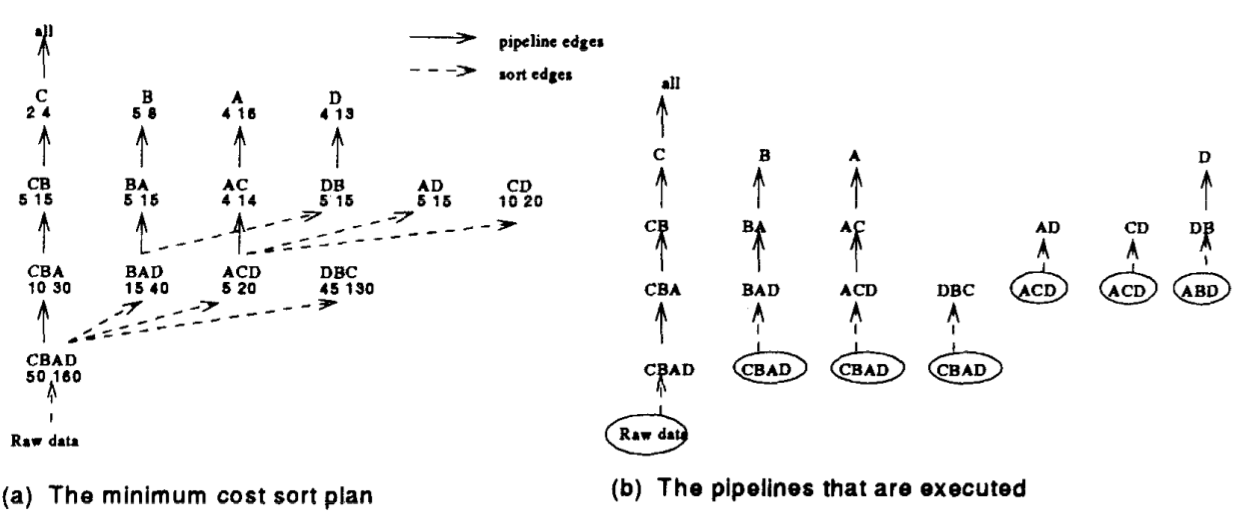
\includegraphics[width=5in]{picture/ch_current_research/pipesort} 
\caption{4维数据立方 pipesort 计算过程}\label{pipesort} 
\end{figure} 

\subsection{PipeHash}

Agarwal 等人还提出了 PipeHash[19]算法,该算法是 PipeSot 算法的一个变形,基于 Hash(散列)实现的。PipeHash 算法首先会根据 GBLP 算法的思想将一个 lattice 修剪成一棵 lattice 执行树。为了使得在同一个聚集计算里的所有元组能够在内存上是相邻的,PipeHash 会为每一个计算的region维护一个散列表。假如有些region的散列表不能同时存放在内存里,则 PipeHash 算法就会把一个 lattice 执行树划分成多棵子树,使得每棵子树内所有region的 Hash表都能够同时存储于内存中。 由于划分代价要比排序代价要小,所以PipeHash 的性能要比 PipeSort 要高。但 PipeSort 用一个排序可以计算多个聚集结果,而 PipeHash 则每次都需要对数据进行重新计算散列值,且 PipeHash 相对于PipeSort 需要大量的内存来存储每棵子树内所有region的散列表。

\subsection{Partitioned-Cube}

以上提到的几种算法都没有考虑到数据稀疏的情况,在现实应用中,事实表往往是稀疏的。针对基于稀疏基表的数据立方的计算 ,Ross 等人在1997 年提出了 Partitioned-Cube 算法 \cite{ross1997fast}。该算法采用分治的策略,对不能完全存储于内存的数据集根据某个候选聚集维属性进行划分,划分成多个子集,因为数据是稀疏的,所以每个子集均能在内存中计算,通过此次划分能够计算所有和该维属性相关的region结果。完成计算后,将该划分维从候选聚集维中去除,根据上述方法重复计算基于剩余维属性的region结果直至数据立方计算完毕。相对于前几种算法,这种算法在数据稀疏的情况下具有更小的 I/O 代价,且受维度增加的性能影响较少。图\ref{partitioned_cube} 为 4 维数据使用 Partitioned-Cube 计算的过程。

\begin{figure}[!htb]
\centering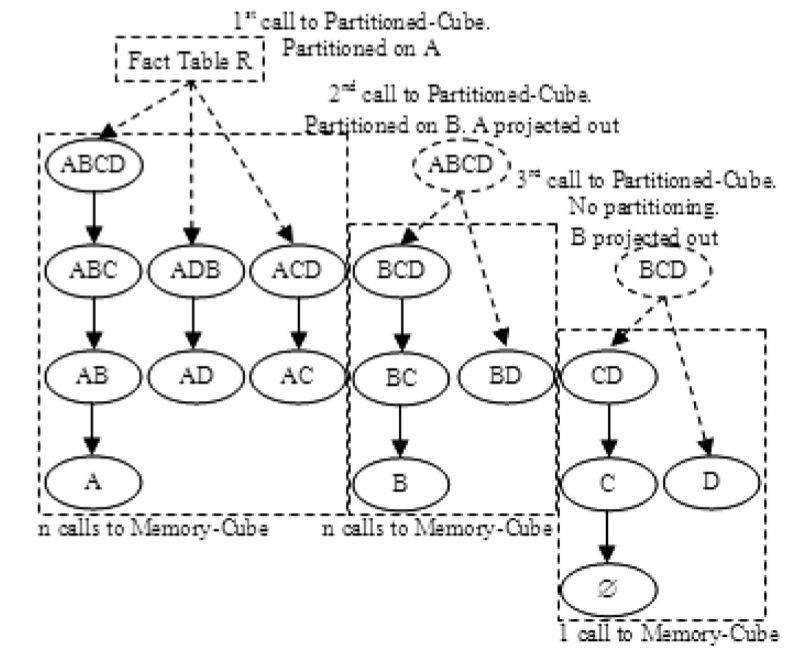
\includegraphics[width=3.5in]{picture/ch_current_research/partitioned_cube} 
\caption{Partitioned Cube 的计算过程}\label{partitioned_cube} 
\end{figure} 

\subsection{BUC}

相对于上述几种自顶向下的数据立方计算算法,Beyer 等人在 1999 年提出的 BUC (Bottom Up Cube) 则是一种自底向上的算法。BUC 算法是在 Partitioned-Cube 算法的思想上,针对冰山数据立方,即基于某个最少阈值的 GroupBy 计算而提出的,也即具有 HAVING 条件的 GroupBy。例如 HAVING COUNT(*) > 100 这样的条件限制。大部分的度量函数是具有单调性的,例如 COUNT(),若 GroupBy(A=a0) 的结果是小于 100,那么 GroupBy(A=a0, B=b0) 的结果必然是小于 100。正是这种单调性,加上有阈值限制,将数据立方的计算变成自底向上,可以实现一定的剪枝。例如上述的例子 COUNT(*) > 100,如果 GroupBy(A=a0)是小于 100 的,那么与 A=a0 相关的 group 就不需要计算了。

BUC算法会根据聚集维属性对基表数据进行多次分组并计算聚集结果,且会基于维顺序对分组进行进一步的细分计算。因为在计算过程中考虑了阈值的问题,所以从 lattice 的底部越往上,region需要进行聚集计算的数据就会变得越少。图 \ref{BUC_partition} 是 BUC 根据属性 A 进行的划分。图 \ref{BUC_execution} 是 BUC 的执行过程。在图 \ref{BUC_execution} 中,原数据分别按照 A, B, C, D 这4个属性进行划分。在属性 A 的划分中,计算所有与属性 A 相关的region,当出现一个region不满足阈值时,则往上的region都不需要计算了。BUC 相比与 PipeSort 和 PipeHash 相比,非常适合有阈值限制的数据立方计算。但将 BUC 用于没有阈值限制的数据立方计算上,它也会有I/O 代价问题。

\begin{figure}[!htb]
\centering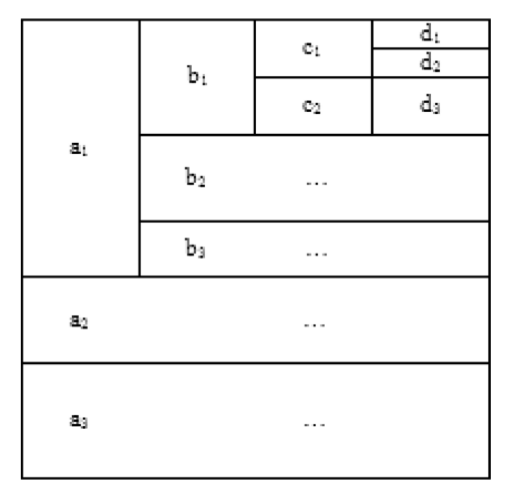
\includegraphics[width=1.7in]{picture/ch_current_research/BUC_partition} 
\caption{BUC 使用维属性的划分}\label{BUC_partition} 
\end{figure} 


\begin{figure}[!htb]
\centering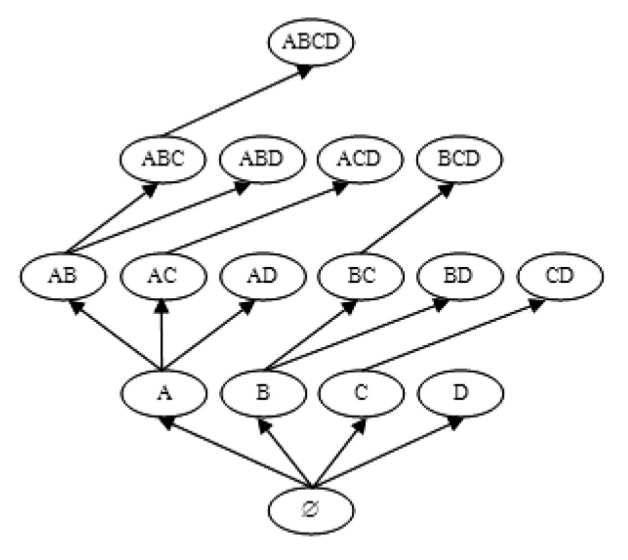
\includegraphics[width=3in]{picture/ch_current_research/BUC_execution} 
\caption{BUC 的执行过程}\label{BUC_execution} 
\end{figure} 


%\section{部分数据立方的计算研究}

%在前文提到,当一个数据立方的维度为 D 时,数据立方内就包含了 ${2}^{D}$ 个region,也即 ${2}^{D}$ GroupBy  计算。当维度增加时,数据立方的计算和存储代价就会呈指数增长。在现实条件下,计算时间和存储空间往往都受限制,而且对于某些region,在现实中也常常不是 OLAP 分析人员需要的数据。因此可选择只计算部分的数据立方,在这里提到的部分数据立方,是指在立方实现与存储时选择了部分region而非所有region的数据立方。当查询的region已计算,则可直接查询获得;若查询的数据region未计算,则从已计算的region中计算获得,而非原数据。于是,如何合理的选择部分立方进行计算就成了部分数据立方计算实现和提高查询相应速度的关键。

%Harinarayan 等人在1996 年提出的贪心算法 BPUS \cite{harinarayan1996implementing} ,通过单位空间效益的指标来对region节点进行贪心选择。该算法比穷尽搜索要快,但算法复杂度较高,随立方维度增加算法时间复杂度呈指数增长。 Shukla等人在 1998 年基于 BPUS 算法思想提出了一个使用简单启发式搜索的改进算法 PBS \cite{shukla1998materialized} ,该算法时间复杂度较低,其运行速度比 BPUS 要快几个数量级,且它能够容易的与自底向上的立方计算方法整合,但该算法会为了加快其运行速度而牺牲了一定的结果质量。除了从存储与计算代价角度来考虑region的选择外,业界也尝试从立方维护代价等多个角度进行region选择算法的设计与优化。

\section{分布式数据立方的计算研究}

随着数据集的大小和维度的数量呈现极速增长,单机的内存和计算力无法满足数据立方的计算要求。因此业界开始研究利用分布式计算的优势实现数据立方的方法。\cite{nandi2011distributed} \cite{dehne2006cgmcube} \cite{ng2001iceberg} \cite{lee2012efficient}。

\cite{ng2001iceberg} 中提出了在由一定数量的 PC机 组成的集群上计算数据立方的方法,包括了RP、BPP、ASL、PT。因为该论文提出的实现环境是集群,因此这4种方法都涉及如何将计算分配到多个节点上。以下简单地阐述这4种方法。

\begin{itemize}

\item \textbf{RP(Replicated Parallel BUC)}

RP 对计算的划分非常简单,基本与 BUC 相似,若有 m 个维属性,则将计算划分为 m 个子任务。每个任务处理与一个维属性相关的所有region的计算。如图 \ref{cluster_rp} 所示,图中因为共有 4 个维属性 ABCD,因此可将计算划分为 4 个子任务,分别计算从维属性 A,B,C,D 出发的各个region。

\begin{figure}[!htb]
\centering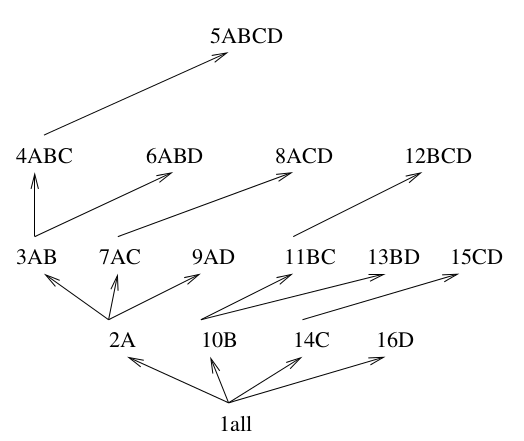
\includegraphics[width=3in]{picture/ch_current_research/cluster_rp} 
\caption{RP 的任务划分图}\label{cluster_rp} 
\end{figure} 

\item \textbf{BPP(Breadth-first writing, Partitioned, Parallel BUC)}

RP 的划分非常简单,同时也存在非常严重的负载均衡问题,有一些任务需要进行大量的计算,如图 \ref{cluster_rp} 中的维属性 A 对应的任务,而有一些则只需要进行非常少量的计算,如 D。BPP 则可以解决该问题。BPP 借鉴了 \cite{ross1997fast} 中的 Partitioned-Cube 算法。

对于一个属性 ${R}_{i}$,根据其属性值的范围,将数据集划分为 n 个子块,而 n 正是节点的数量。对于每个属性都继续进行类似的划分操作。因此,若有 m 个维属性,则有 $n \times m$ 个子块。多个属性的子块划分可同时进行,最后将这些子块分发到各个节点上计算相应的region。

这样的方法比 RP 相比,负载均衡的问题就减轻不少。

\item \textbf{ASL(Affinity SkipList)}

ASL 使用跳表来维护region内的数据。跳表的一个重要特征是其有序性。因此若对region ABCD 维护了一张跳表,则可从调表上计算 ABC,AB,A 这三个region。这个与 Pipesort 类似。若要计算的region并没有建立跳表,但它是已建立跳表的region的后缀,则仍可从已建立的跳表中较快速地计算。如region BCD 可从 ABCD 中计算获得,相比从原数据中计算获得有更高的效率。如果以上两种情况都不满足,只能重新构建跳表。
 
\item \textbf{PT(Partitioned Tree)}

PT 是对 lattice 不断使用二分划分的方法,直到划分的子 lattice 的数量与节点数量相同则停止。图 \ref{cluster_pt} 是 PT 的任务划分图。

\begin{figure}[!htb]
\centering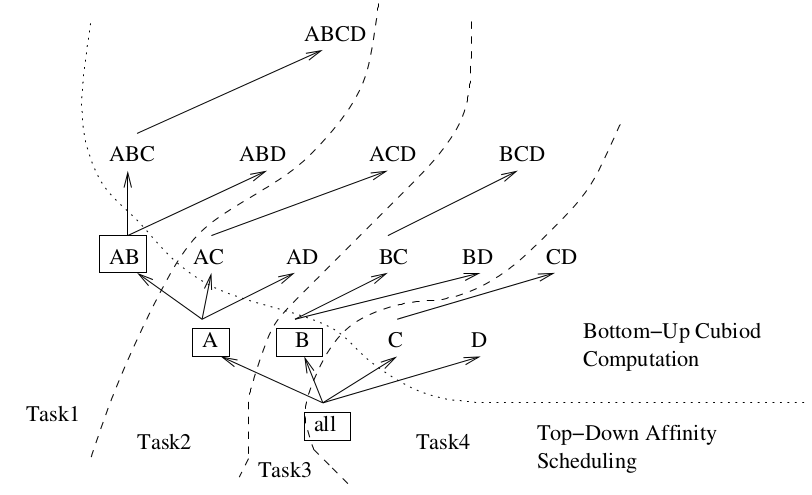
\includegraphics[width=4in]{picture/ch_current_research/cluster_pt} 
\caption{PT 的任务划分图}\label{cluster_pt} 
\end{figure} 

\end{itemize}


cgmCUBE \cite{dehne2006cgmcube}、RP、BPP、ASL、PT\cite{lee2012efficient} 这几个算法是基于由少量 PC 机组成的集群实现的,并没有与 MapReduce 框架相结合。 \cite{you2008parallel} \cite{sergey2009applying} 虽将数据立方的计算与 MapReduce结合,但无法很好地处理整体性度量函数的计算,也并没有考虑到数据倾斜的情况。

MR-Cube \cite{nandi2011distributed} 是基于 MapReduce 提出的数据立方算法,该算法结合了 MapReduce 与数据立方计算的特点,能够达到高效实现 TB 级数据量的数据立方计算。MR-Cube 针对整体性度量函数提出了相应的分布式计算思路,并指出了其中 2 种整体性度量函数实际的分布式计算处理方法。 为了避免MapReduce 集群节点间的数据分布不均衡,MR-Cube 采用对数据进行采样的方法来决定如何在后续计算中对region进行切割以使得集群节点间装载平衡。利用数据立方region间计算过程可共享的特性, MR-Cube 对数据立方lattice 进行划分,使得每个分支能在共享一套数据的基础上进行 BUC 计算,从而降低了 MapReduce 处理的中间数据量。

虽然 MR-Cube 是目前基于 MapReduce 框架一个较好的数据立方实现。但MR-CUBE 现有的一些不足不得不提。MR-Cube 的数据划分是基于整个region的,当region内某个group的计算数据过度倾斜,而其他group的计算数据都较小时,对整个region进行划分就会导致一些group不必要的划分。过多的划分会导致后续的合并计算过多,当数据过度倾斜时,这种划分方式的劣势就会十分明显。并且在 lattice 分支上使用 BUC 的计算,没有充分利用 MapReduce的特性,BUC 需要对数据扫描多次,这样将导致多次I/O或者需要将数据都载入内存。

由于本文的主要工作是对 MR-Cube 进行改进,因此关于 MR-Cube 主要的贡献和存在的不足将在下一章详细说明。



